\chapter{Event selection in ND-GAr}
\label{chapter:gar_selection}

\section{Data sample}

\begin{table}[t]
	\caption{Event rates in ND-GAr.}
	\begin{center}
		\begin{small}
			\begin{tabular}{lcc}
                & \multicolumn{2}{c}{Events/ton/year}                                                                   \\[2mm] \cline{2-3} 
            \multicolumn{1}{c}{\rule{0pt}{1.1\normalbaselineskip}Process}       & $1.1 \times 10^{21} ~ \mathrm{POT}/\mathrm{year}$ & $1.9 \times 10^{21} ~ \mathrm{POT}/\mathrm{year}$ \\[2mm] \hline
            \rule{0pt}{1.1\normalbaselineskip}All $\nu_{\mu}$-CC                & $1.60 \times 10^{6}$                              & $2.83 \times 10^{6}$                              \\[2mm]
            $\hspace{0.5 cm}$ CC $0\pi$       & $5.28 \times 10^{5}$                              & $9.35 \times 10^{5}$                              \\[2mm]
            $\hspace{0.5 cm}$ CC $1\pi^{\pm}$ & $3.02 \times 10^{5}$                              & $5.34 \times 10^{5}$                              \\[2mm]
            $\hspace{0.5 cm}$ CC $1\pi^{0}$   & $1.65 \times 10^{5}$                              & $2.92 \times 10^{5}$                              \\[2mm]
            $\hspace{0.5 cm}$ CC $2\pi$       & $3.18 \times 10^{5}$                              & $5.63 \times 10^{5}$                              \\[2mm]
            $\hspace{0.5 cm}$ CC $3\pi$       & $1.36 \times 10^{5}$                              & $2.41 \times 10^{5}$                              \\[2mm]
            $\hspace{0.5 cm}$ CC other        & $1.52 \times 10^{5}$                              & $2.69 \times 10^{5}$                              \\[2mm] \hline
            \rule{0pt}{1.1\normalbaselineskip}All $\bar{\nu}_{\mu}$-CC          & $7.54 \times 10^{4}$                              & $1.33 \times 10^{5}$                              \\[2mm]
            All NC                            & $5.50 \times 10^{5}$                              & $9.73 \times 10^{5}$                              \\[2mm]
            All $\nu_{e}$-CC                  & $2.70 \times 10^{4}$                              & $4.78 \times 10^{4}$                             
            \end{tabular}
		\end{small}
	\end{center}
	\label{tab:ndgar_event_rates}
\end{table}

\section[\texorpdfstring{$\nu_{\mu}$}{numu} CC selection]{\boldmath\texorpdfstring{$\nu_{\mu}$}{numu} CC selection}

In a $\nu_{\mu}$ CC inclusive selection, the signal topology we look for is a neutrino-induced muon with or without other final state particles. Here, I also require the neutrino vertex to be located inside the fiducial volume (FV) of ND-GAr.

The FV is defined as a smaller cylinder within the cylindrical volume of the HPgTPC. The FV has a radius $R_{\mathrm{FV}}$ and a half-length $L_{\mathrm{FV}}$. For a particle position to lie within the FV it must satisfy:
\begin{equation}
    \vec{x}_{i} \in \left\{\vec{x} \in \mathbb{R}^{3} \mid |x_{0}| \leq L_{\mathrm{FV}} ~ \& ~ \sqrt{x_{1}^{2}+x_{2}^{2}} \leq R_{\mathrm{FV}}\right\},
\end{equation}
in the reference frame of the HPgTPC. For convenience, I define:
\begin{equation}
    \begin{split}
        \Delta R_{\mathrm{FV}} &= R_{\mathrm{HPgTPC}} - R_{\mathrm{FV}}, \\
        \Delta L_{\mathrm{FV}} &= L_{\mathrm{HPgTPC}} - L_{\mathrm{FV}},
    \end{split}
\end{equation}
where $R_{\mathrm{HPgTPC}}$ and $L_{\mathrm{HPgTPC}}$ refer to the radius and the half-length of the HPgTPC, respectively. Figure \ref{fig:ndgar_ana_geometry} shows the HPgTPC volume with the FV inside of it. In that representation, the FV is defined as $\Delta L_{\mathrm{FV}} = 30.0 ~ \mathrm{cm}$ and $\Delta R_{\mathrm{FV}} = 30.0 ~ \mathrm{cm}$. Also shown is the HPgTPC reference frame, with $x$ being the drift direction and $z$ aligned along the beam direction.

In some cases, it is interesting to divide the signal events in different categories based on their true interaction mode. In this work, I will distinguish between charged-current quasi-elastic (CCQE), coherent (CCCOH), resonant (CCRES), and deep-inelastic (CCDIS) interactions. I also use a separate category for the interactions not included in any of the other categories (CCOther).

Any other events are considered backgrounds. For this selection, I use the following categorisation of background events:
\begin{itemize}
    \item Out of FV: if the true neutrino vertex lies outside the defined FV.
    \item NC: if the event is a true neutral-current event.
    \item $\bar{\nu}_{\mu}$ CC: if the true neutrino candidate is of muon antineutrino flavour.
    \item Other: if the event is not signal nor falls in any of the other background categories.
\end{itemize}

\begin{figure}[t]
\centering
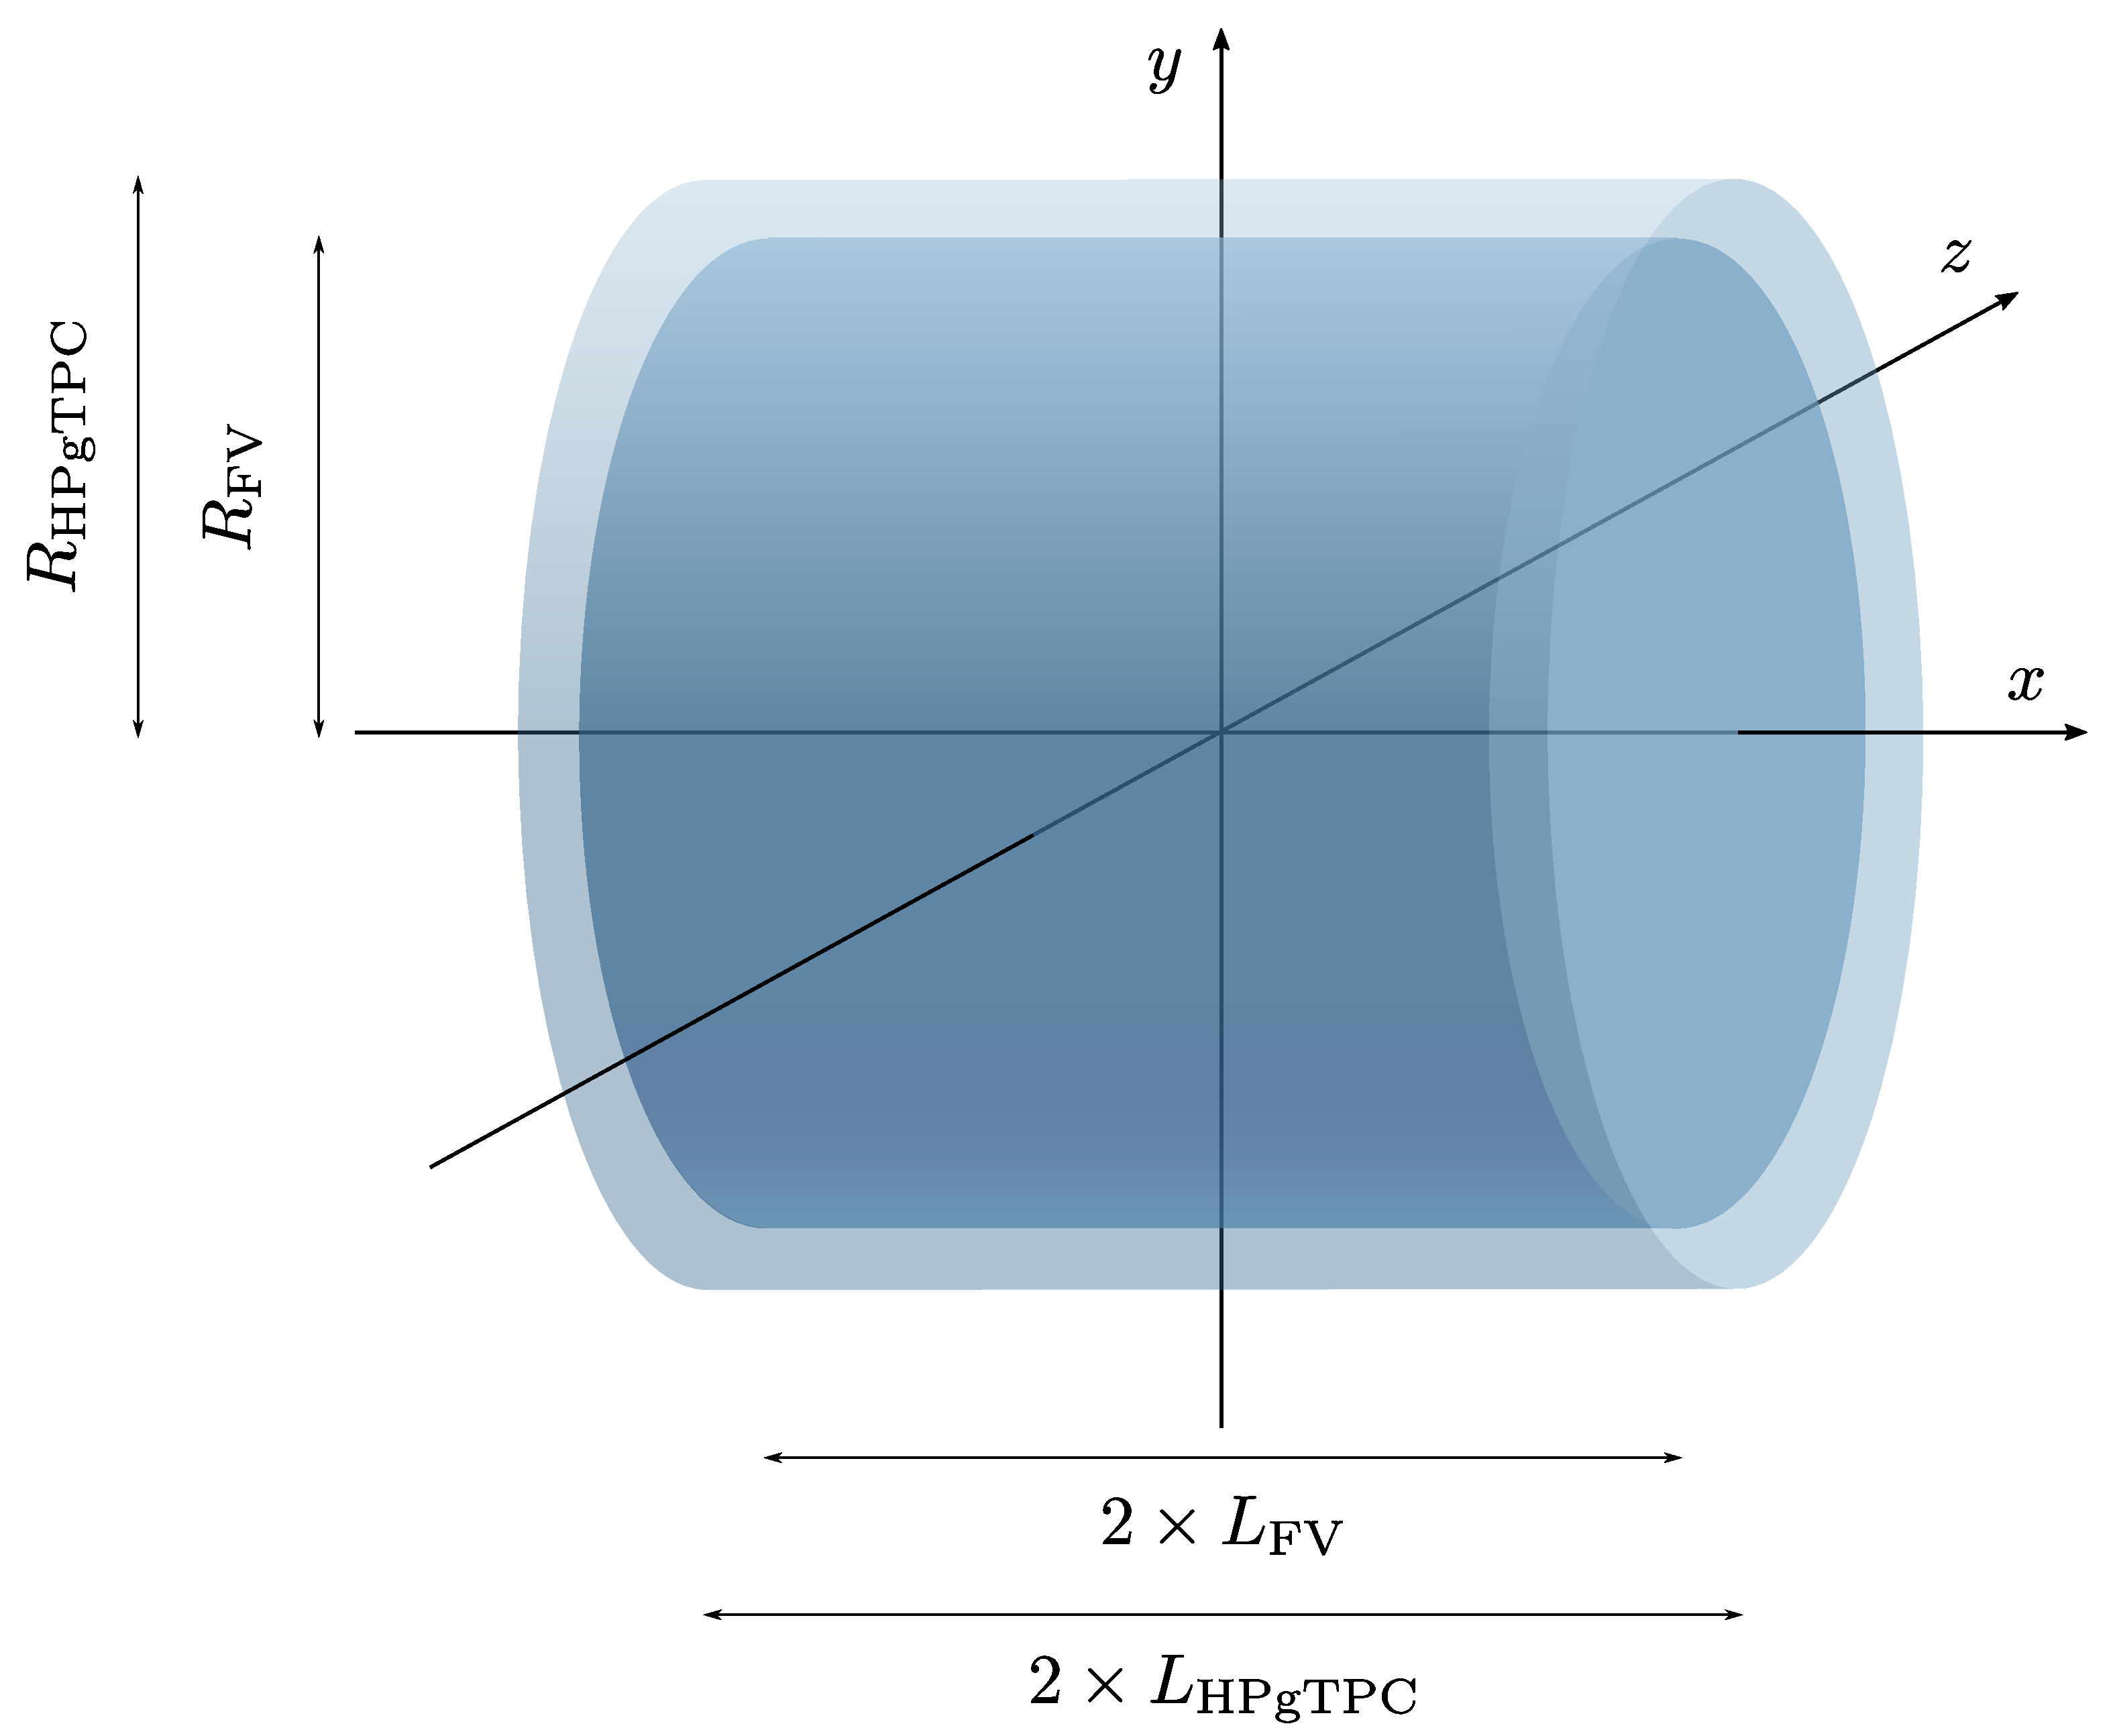
\includegraphics[width=.90\linewidth]{Images/GAr_selection/ndgar_ana_geometry.pdf}
\caption[Schematic diagram of the HPgTPC including the fiducial volume.]{Schematic diagram of the HPgTPC including the fiducial volume (FV). In this case the FV is given by $\Delta L_{\mathrm{FV}} = 30.0 ~ \mathrm{cm}$ and $\Delta R_{\mathrm{FV}} = 30.0 ~ \mathrm{cm}$.}
\label{fig:ndgar_ana_geometry}
\end{figure}

The key to the CC selection is the identification of a primary muon candidate. Typically, this is the longest track in the event. However, sometimes protons and pions leave tracks longer than that of the muon. This is particularly important in the GAr medium, considerably less dense than the LAr. For this reason, the muon identification in ND-GAr relies heavily on the capabilities of the ECal.

The selection strategy proposed combines the information coming from the three main detection systems of ND-GAr: the HPgTPC charge readout, and the ECal and $\mu$ID detectors. It consists of five steps:
\begin{enumerate}
    \item Event contains reconstructed particles.
    \item Select particles with reconstructed negative charge, $q_{\mathrm{reco}} = -1$.
    \item Select particles passing the muon score cut, $\mu_{\mathrm{score}} \geq \mu_{\mathrm{score}}^{\mathrm{cut}}$.
    \item Keep reconstructed particle with the highest momentum, $\mathrm{max}\left[p_{\mathrm{reco}}\right]$.
    \item Check that the remaining particle starts within the FV.
\end{enumerate}
All the events passing these cuts are classified as signal, and the selected particle is regarded as the primary muon candidate.

\subsection{Selection optimisation}

I performed an optimisation of the selection . For the muon selection, I varied the value of $\mu_{\mathrm{score}}^{\mathrm{cut}}$ from $0.05$ to $0.95$, using a step size of $0.05$. Additionally, to optimise the FV, I systematically explored a number of different parameter configurations, moving within the $10.0-70.0~\mathrm{cm}$ range for $\Delta L_{\mathrm{FV}}$ and $25.0-75.0~\mathrm{cm}$ for $\Delta R_{\mathrm{FV}}$, in increments of $10.0~\mathrm{cm}$ and $5.0~\mathrm{cm}$ respectively.

For each parameter configuration, I extract three different true neutrino energy distributions. These are built combining the results of the selection described previously, which we can refer to as the ``reco'' selection, and a ``true'' selection. The later identifies the true $\nu_{\mu}$ CC events using the GENIE event records, and checks that the true neutrino vertices are contained in the FV.

The first distribution consists of the events passing both selections, i.e., these are the true $\nu_{\mu}$ CC events which pass the ``reco'' selection. The second distribution of the events passing the ``reco'' selection but failing the ``true'' selection. These are the background events that the selection misidentifies. Finally, the third distribution corresponds to the events 

\begin{figure}[t]
    \centering
    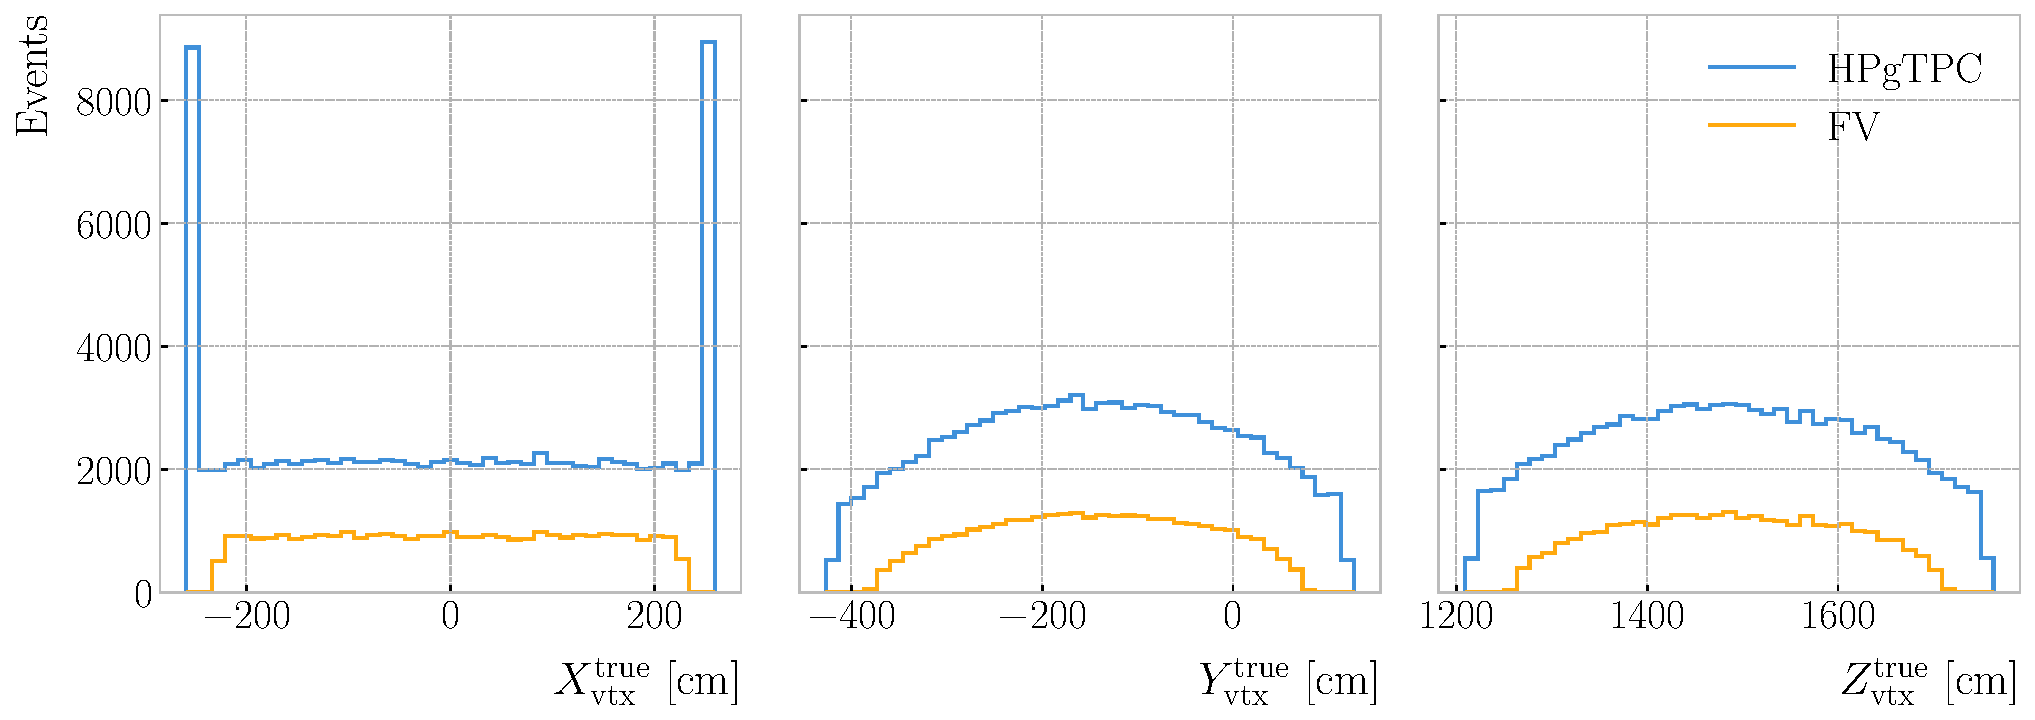
\includegraphics[width=.99\linewidth]{Images/GAr_selection/numuCC_true_vertex_position_fiducial.pdf}
    \caption[Distributions of the true $\nu_{\mu}$ CC vertex positions for the full HPgTPC and the FV.]{Distributions of the true $\nu_{\mu}$ CC vertex positions for the full HPgTPC volume (blue) and the optimised FV (yellow), given by $\Delta L_{\mathrm{FV}} = 30.0 ~ \mathrm{cm}$ and $\Delta R_{\mathrm{FV}} = 50.0 ~ \mathrm{cm}$.}
    \label{fig:numuCC_true_vertex}
\end{figure}

\begin{table}[t]
	\caption[Step-by-step $\nu_{\mu}$ CC selection cuts and cumulative passing rates.]{Step-by-step $\nu_{\mu}$ CC selection cuts and cumulative passing rates. Relative passing rates are indicated in parentheses.}
	\begin{center}
		\begin{small}
			\begin{tabular}{c|ccc}
                Cut \# & Selection cut                       & Events & Passing rates          \\[2mm] \hline
                \rule{0pt}{1.1\normalbaselineskip}0      & Total number of events (No cuts)    & 100000 & $100.00\% ~(100.00\%)$ \\[2mm]
                1      & At least one reconstructed particle                              & 85680  & $85.68 \% ~(85.68 \%)$ \\[2mm]
                2      & Negatively charged particles only                                & 62054  & $62.05\% ~(72.43\%)$   \\[2mm]
                3      & $\mu_{\mathrm{score}} \geq \mu_{\mathrm{score}}^{\mathrm{cut}}$  & 45035  & $45.03\% ~(72.57\%)$   \\[2mm]
                4      & Candidate $\vec{x}_{\mathrm{start}}$ in FDV                      & 31212  & $31.21\% ~(69.31\%)$  
                \end{tabular}
		\end{small}
	\end{center}
	\label{tab:numuCC_selection}
\end{table}

\begin{figure}[t]
	\centering
	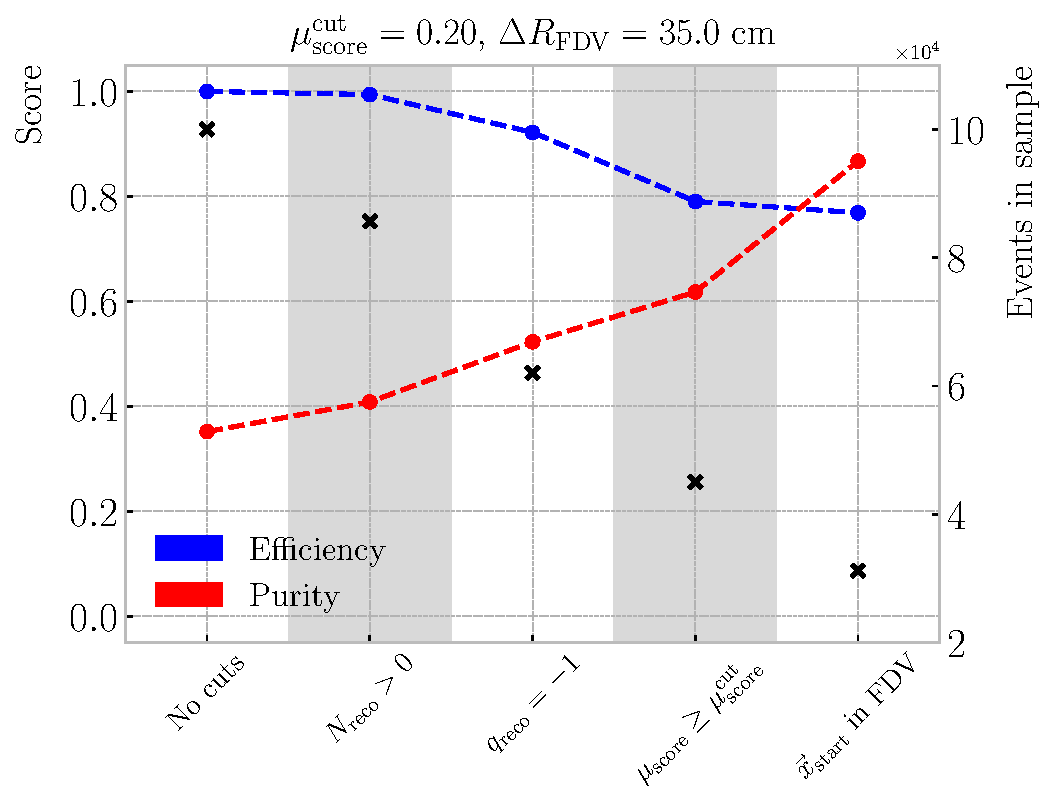
\includegraphics[width=.90\linewidth]{Images/GAr_selection/numu_cc_selection_steps.pdf}
	\caption[Cumulative efficiency and purity of the $\nu_{\mu}$ CC selection.]{Cumulative efficiency (blue) and purity (red) of the $\nu_{\mu}$ CC selection. Also indicated is the number of events in the sample after each cut (black crosses).}
	\label{fig:numuCC_selection_steps}
\end{figure}

\subsection{Primary muon kinematics}

\section{Charged pion identification}

\subsection[\texorpdfstring{$\nu_{\mu}$}{numu} CC \texorpdfstring{$1\pi^{\pm}$}{1pi} selection]{\boldmath\texorpdfstring{$\nu_{\mu}$}{numu} CC \boldmath\texorpdfstring{$1\pi^{\pm}$}{1pi} selection}